% Drawing 80/01-6 -- folder 80, batch 01, archive page 13 (PDF page 14).
% Transcription: en haut de la carte, deux petites figures à l'encre : à gauche un carré, deux coins du haut marqués « $-1$ » et « $+1$ », recoupé par une diagonale épaisse, des traits en tirets et une droite oblique venue du haut à gauche, un point marqué sur son côté supérieur ; à droite un carré analogue, traversé d'une longue droite oblique épaisse et de plusieurs traits repassés
% Kind: two small sketches: squares cut by oblique lines. Method 2 (schematic redraw from the facsimile). Status: ok.
% Notes: Two free-hand ink sketches, redrawn stroke by stroke. Left: the square, an inner smaller square at its upper left, the dashed horizontal and vertical, the heavy diagonal from the left side, a pencil stroke parallel to it, the heavy dot on the top side with a heavy stroke to the right side, the long oblique line from the upper left (doubled) and short strokes beside it; the corner labels are read -1 and +1 (the transcription's note has two corners marked with a double prime). Right: the square, the long heavy oblique line through it, the dashed horizontal and vertical inside, several oblique strokes gone over, dashes at the upper left. Left out: faint pencil ovals over the right square. Still differs: both are overdrawn several times; the strokes are a reading and their ends are approximate. Redrawn 2026-11-12 (issue 128): to check again. 2026-11-14, Claude Opus 5.5, overlay check (issue 147): rasterised from its own coordinates over the 400 dpi colour scan, laid over it at 22 to 28 px per unit, corrected and measured (all ink of the two figures within 1.5 units of a stroke); not compiled (no TeX in the session). Changed: in the left square the dashed horizontal runs on to the right side, as on the page; in the right figure the short dashed stroke at the upper left was a solid stroke doubling the heavy oblique below it, from its top down to the first dashes, and is drawn so; a short stroke there moved 2 units right onto its ink. Added: the small heavy V-shaped mark in ink between the two figures (not in the transcription; it may be a letter). The other strokes, the dot and the corner labels lie on their ink to within about 1 unit; the overdrawn strokes are drawn one by one as they lie. Left out, as before: the faint pencil ovals over the right square. Status set to ok.
% Coordinates: 1 unit = 1 mm = 1/100 of the crop width (bbox in page fractions: [0.17, 0.07, 0.88, 0.255]).
% Redrawn by Claude (claude-fable-5-2), issue #128, 2026-11-12; not checked by a human; not compiled (no TeX in the session).
% Checked by Claude (claude-opus-5-5) 2026-11-14 (issue #147): overlaid on the 400 dpi colour facsimile, corrected; not compiled (no TeX in the session). Not checked by a human. Status: ok.
% Rights: reproduces part of the work -- behind RENDER_TRANSCRIPTS, never published by itself.
\documentclass[tikz,border=3pt]{standalone}
\usepackage{amsmath,amssymb}
\usetikzlibrary{patterns,arrows.meta}
\tikzset{pencil/.style={black!45}, struck/.style={black!35}, mpt/.style={circle,draw,inner sep=1.3pt}, pt/.style={circle,fill,inner sep=0.9pt}, opt/.style={circle,draw,fill=white,inner sep=1.1pt}}
\begin{document}
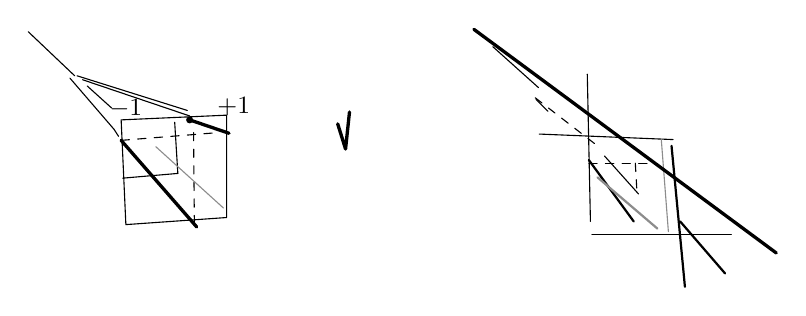
\begin{tikzpicture}[x=1mm,y=1mm,line cap=round,line join=round,font=\scriptsize]
\draw (13.3,-13.7) -- (26.7,-13.1) -- (26.7,-26.1) -- (13.9,-27) -- (13.3,-13.7);
\draw[dashed] (13.3,-16.3) -- (25.8,-15.3);
\draw[dashed] (22.5,-15.3) -- (22.6,-27);
\draw (20.1,-14) -- (20.5,-20.5);
\draw (13.5,-21.1) -- (20.5,-20.5);
\draw[very thick] (13.3,-16.3) -- (22.9,-27.3);
\draw[pencil] (17.7,-17.1) -- (26.3,-24.9);
\draw[very thick] (22,-13.7) -- (27,-15.4);
\node[pt] at (22,-13.7) {};
\draw (1.5,-2.5) -- (7.4,-8.1);
\draw (7.7,-8.1) -- (21.7,-12.5);
\draw (8.4,-8.6) -- (22,-13.2);
\draw (6.8,-8.4) -- (12.4,-14.9);
\draw (9,-9.4) -- (12.1,-12.2);
\draw[dashed] (12.4,-14.9) -- (13.3,-16.3);
\node[inner sep=1pt] at (13.9,-12.3) {\small $-1$};
\node[inner sep=1pt] at (27.6,-12) {\small $+1$};
\draw (72.5,-7.9) -- (72.9,-26.6);
\draw (66.4,-15.5) -- (83.4,-16.2);
\draw[thick] (83.2,-17) -- (84.9,-34.9);
\draw[pencil] (81.9,-16.2) -- (82.8,-27.9);
\draw (73.1,-28.2) -- (90.8,-28.2);
\draw[dashed] (72.7,-19.2) -- (81.2,-19.2);
\draw[dashed] (78.6,-19.2) -- (78.8,-22.7);
\draw[very thick] (58.1,-2.2) -- (96.5,-30.6);
\draw[thick] (84.3,-26.6) -- (90,-33.2);
\draw[thick] (72.7,-18.8) -- (78.4,-26.6);
\draw (74.7,-18.3) -- (79,-23.1);
\draw[pencil,thick] (73.8,-21) -- (81.4,-27.5);
\draw (60.5,-4.4) -- (66.3,-9.6);
\draw[dashed] (65.9,-10.9) -- (73.8,-17);
\draw (66,-11.1) -- (67.5,-12.6);
\draw[very thick] (40.8,-14.2) -- (41.8,-17.4) -- (42.3,-12.7);
\end{tikzpicture}
\end{document}
